\section{Uživatelské rozhraní}

Dle rešerše konkurenčních aplikací je cílem návrhu uživatelského rozhraní
vytvořit jednoduchou grafiku,
ve které se bude snadno navigovat a~kterou uživatel snadno pochopí.
Pro návrh uživatelského rozhraní je využíváno wireframů,
což je metoda pro návrh rozhraní,
kdy je obrazovka naskreslena pomocí jednoduchých tvarů
a~je tedy zobrazována struktura dané obrazovky,
místo konkrétního zpracování.
To slouží pro vyjádření základní reprezentace rozložení,
které ovšem nemusí být finální a~výsledná podoba obrazovek se může lišit. 
Veškeré wireframy byly vytvořeny pomocí programu draw.io.

V~následujících sekcích jsou popsány obrazovky jednotlivých modulů
s~obrázkami daných wireframů.

\subsection{Modul home}

Modul home slouží pro navigaci uživatele mimo hru samotnou.
Návrh tohoto modulu je velmi důležitý,
jelikož uživatele do samotné aplikace uvede a~umožní další postup.
Cílem návrhu tohoto rozhraní je snadno provést uživatele přihlášením,
registrací, menu, profilem, informacemi o~aplikaci a~nastavením.
Modul obsahuje celkem sedm obrazovek.

\begin{figure}
    \centering
    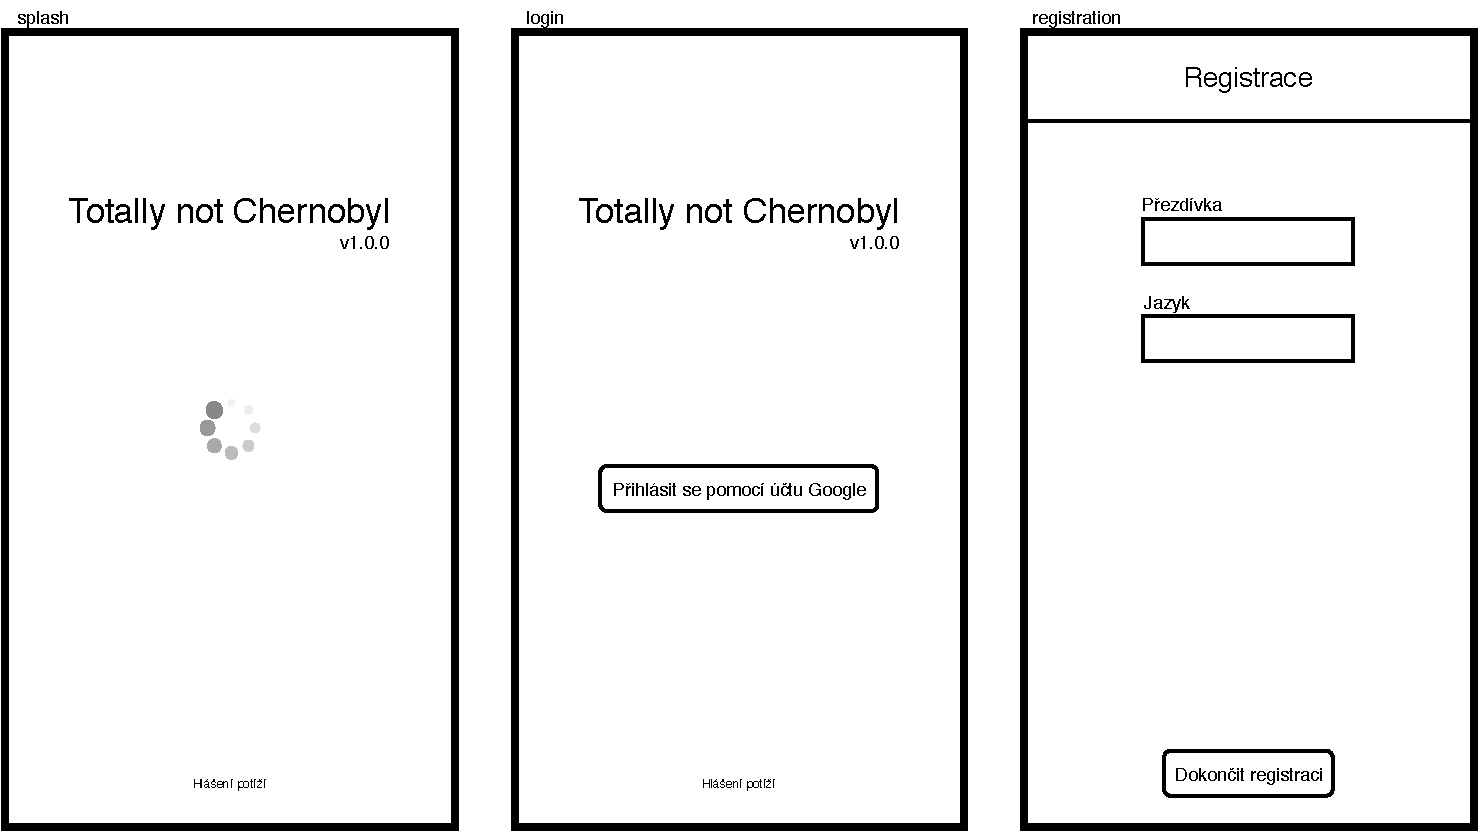
\includegraphics[width=1\linewidth]{assets/design/wireframes/home-1.pdf}
    \caption{Wireframy obrazovek splash, login a~registration}
    \label{fig:ui-home-1}
\end{figure}

Na obrázku~\ref{fig:ui-home-1} lze vidět obrazovky splash,
která slouží pro načítání aplikace,
login,
která slouží pro přihlášení uživatele,
a~registration,
která slouží pro vyplnění informací při registraci nového uživatele.
Tyto obrazovky jsou první,
které uživatel uvidí.
Proto je nutné,
aby byly obrazovky snadno pochopitelné a~jednoduché.
Uživatel na obrazovkách vidí pouze logo a~příslušné ovládací prvky,
což splňuje podmínky na jednoduchost.  

\begin{figure}
    \centering
    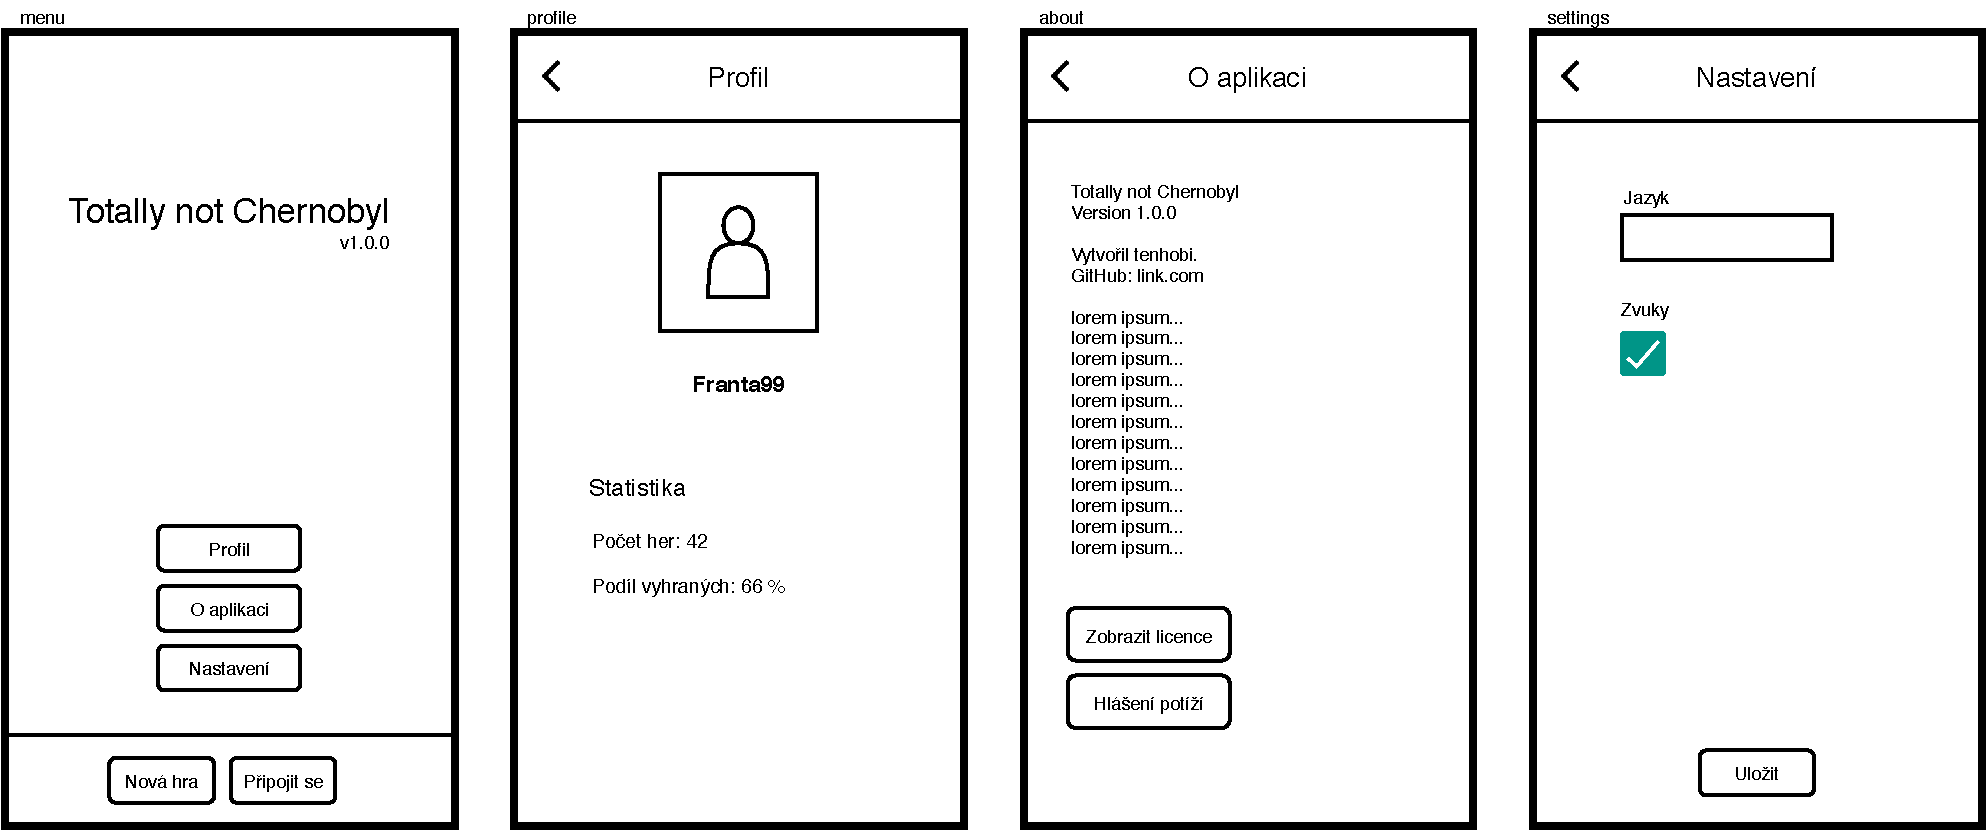
\includegraphics[width=1\linewidth]{assets/design/wireframes/home-2.pdf}
    \caption{Wireframy obrazovek menu, profile, about a~settings}
    \label{fig:ui-home-2}
\end{figure}

Po přihlášení do aplikace se uživatel přesune na obrazovku menu.
Z~této obrazovky se může uživatel přesunout kamkoli v~aplikaci,
a~proto jsou uživateli přehledně poskytnuta tlačítka,
která ho srozumitelně provedou.
Jedním z~nejdůležitějších tlačítek je vytvoření hry,
které je přehledně umístěno do spodní lišty.
Z~této obrazovky se uživatel může dostat na obrazovku profil,
kde jsou zobrazeny informace o~uživateli a~jeho statistiky.
Z~obrazovky menu se lze také prokliknout na obrazovky about a~settings.
Obrazovka about obsahuje informace o~aplikaci,
včetně názvu aplikace, verze, vývojáře a~tak podobně.
Na obrazovce settings může uživatel nastavit novou přezdívku nebo změnit jazyk
aplikace.
Tyto obrazovky lze vidět na obrázku~\ref{fig:ui-home-2}.

\subsection{Modul lobby}

Pro vytvoření hry se musí uživatel přesunout na obrazovky modulu lobby,
kde probíhá samotné nastavení hry před jejím vytvořením.
Na tyto obrazovky se dostane hráč z~modulu home po kliknutí na tlačítko
vytvoření hry nebo připojení se do hry.

\begin{figure}
    \centering
    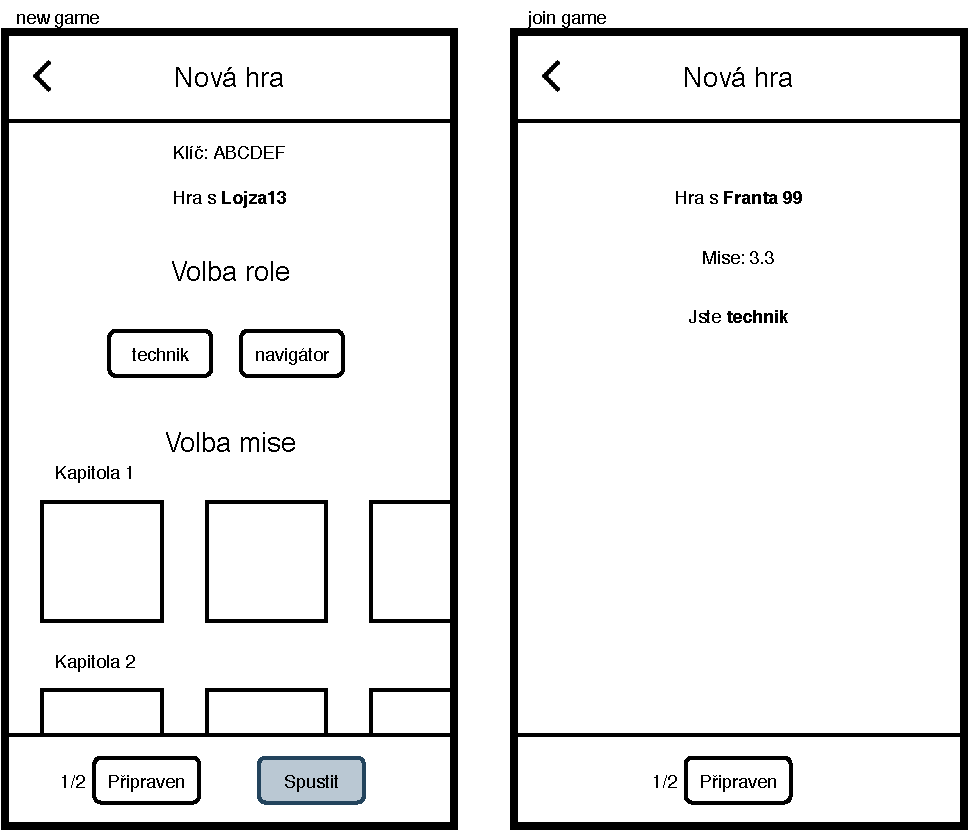
\includegraphics[width=0.6\linewidth]{assets/design/wireframes/lobby.pdf}
    \caption{Wireframy obrazovek new game a~join game}
    \label{fig:ui-lobby}
\end{figure}

Na obrazovce new game může zakládající uživatel nastavit hru,
zejména si zvolit roli a~vybrat misi.
Na obrazovce uživatel vidí klíč pro připojení a~hráče,
který se do hry připojil.
Na dolní liště uživatel přehledně vidí tlačíko na signalizaci ke startu hry
a~k~odstartovánímu samotnému.
Na obrazovce join game vidí uživatel,
který se připojuje do hry,
pouze statické informace o~zvoleném nastavení.
Na dolní liště uživatel přehledně vidí tlačítko na signalizaci ke startu.
Tyto obrazovky jsou zobrazeny na obrázku~\ref{fig:ui-lobby}.

\subsection{Modul game}

Samotný modul hry je složen ze tří obrazovek.
Dvě obrazovky se věnují samotné hře a~zobrazují zbývající čas.
První obrazovka game manual slouží pro zobrazení informací ke vyřešení hry.
Druhá obrazovka je zajímavější.
Obsahuje samotné herní prvky,
mezi kterými musí hráč přepínat a~plnit je.
Třetí obrazovka je obrazovka po skončení hry,
která zobrazuje úspěch či neúspěch
a~statistiky hry.
Tyto obrazovky jsou vidět na obrázku~\ref{fig:ui-game}.

\begin{figure}
    \centering
    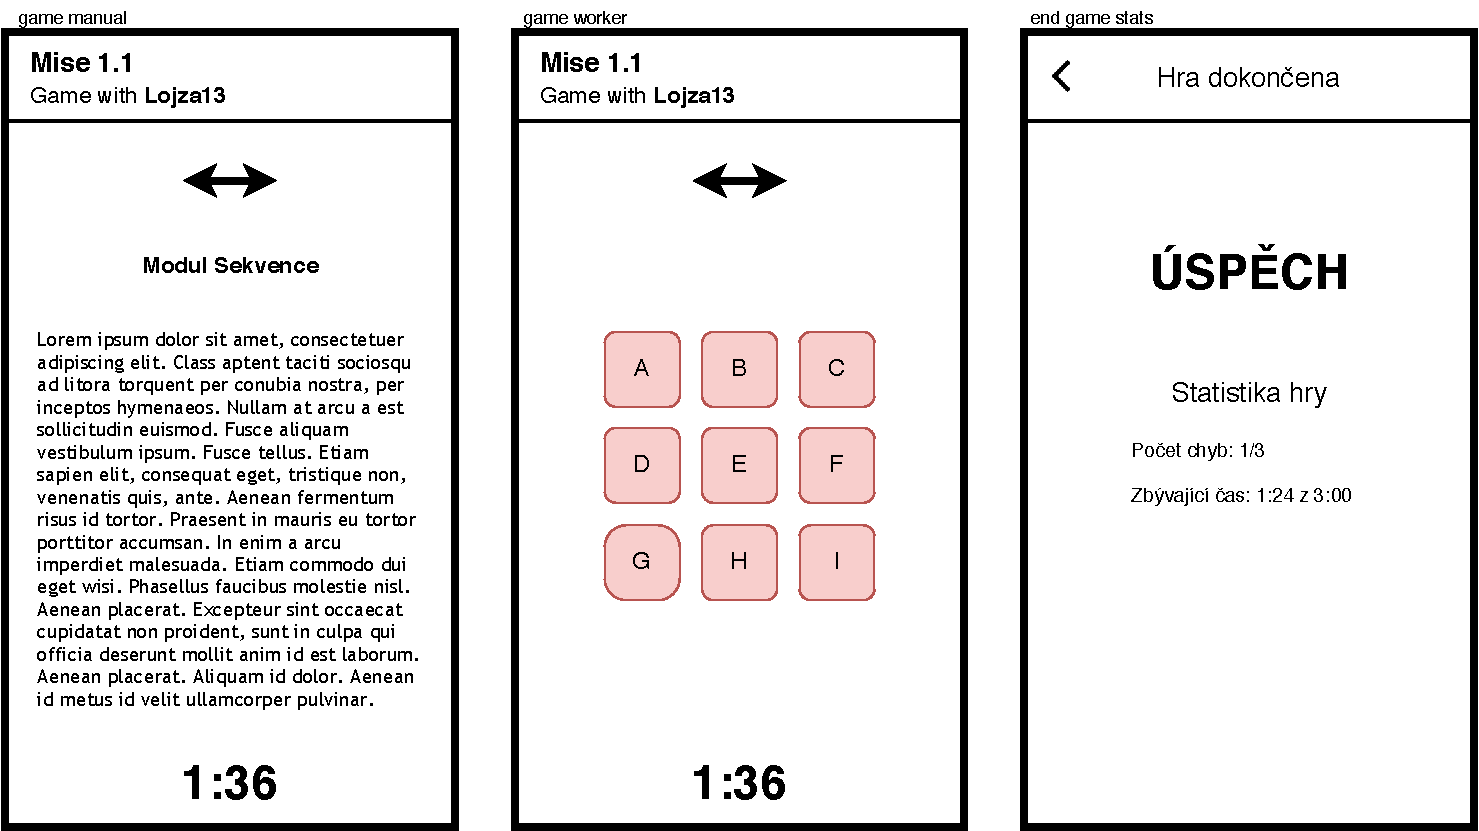
\includegraphics[width=1\linewidth]{assets/design/wireframes/game.pdf}
    \caption{Wireframy obrazovek game manual, game worker a~end game stats}
    \label{fig:ui-game}
\end{figure}
